\section*{Экспериментальные результаты}

\subsection*{Cпектр периодической последовательности прямоугольных импульсов}
Теоретическое описание спектра периодической последовательности прямоугольных импульсов приведено на рисунке \ref{res:impulse}.

\begin{figure}[H]
	\centering
	\begin{minipage}[b]{.49\textwidth}
		\centering
		\includegraphics[width=0.9\linewidth]{"../res/impulse"}
	\end{minipage}%
	\begin{minipage}[b]{.49\textwidth}
		\centering
		\includegraphics[width=0.9\linewidth]{"../res/impulse_spectrum"}
	\end{minipage}
	\caption{Периодическая последовательность импульсов и её спектр.}
	\label{res:impulse}
	\vspace*{-10pt}
\end{figure}

Настраиваем генератор на прямоугольные импульсы с частотой повторения $\nu_T = 1 \; \text{кГц}$ (период $T = 1 \; \text{мс}$) и длительностью импульса $\tau = \frac{T}{20} = 50 \; \text{мкс}$. Снимки экрана электронного осциллографа приведены на рисунках \ref{photo:impulse_nu} и \ref{photo:impulse_tau}. На первом снимке видно, что половина ширины спектра составляет $\Delta \nu = 20$ кГц, что совпадает с рассчитанной выше.

Из соотношения неопределенности $ \Delta \nu \cdot \tau = 1 \Rightarrow \Delta \nu = 20 \; \text{кГц}$, где $\Delta \nu$ -- половина ширины главного спектра.

На снимках \ref{photo:impulse_nu} приведены спектры для различных частот $\nu_T$. Видно, что ширина спектра для них практически не меняется, тогда как меняется расстояние между соседними компонентами спектра.

\begin{figure}[H]
	\centering
	\begin{minipage}[b]{.5\textwidth}
		\vspace*{-10pt}
		\centering
		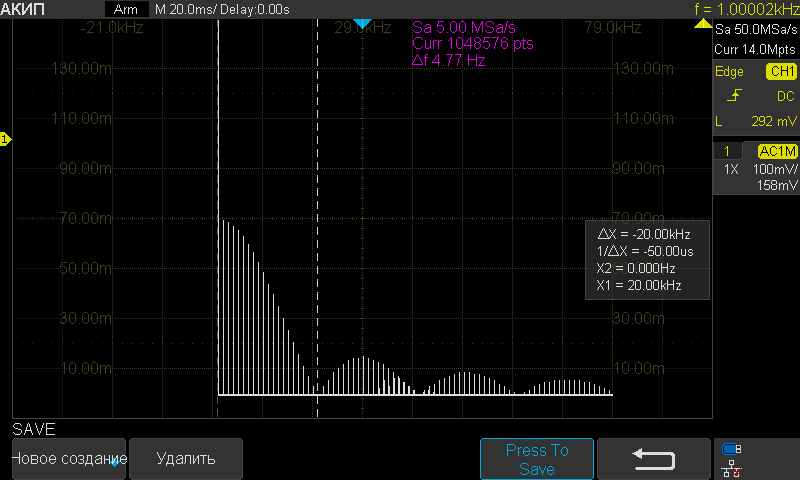
\includegraphics[width=0.9\linewidth]{"../photos/impulse1.png"}
		\vspace*{-5pt}
		\caption*{$\nu_T= 1$ кГц}
		\vspace*{-10pt}
	\end{minipage}%
	\begin{minipage}[b]{.5\textwidth}
		\vspace*{-10pt}
		\centering
		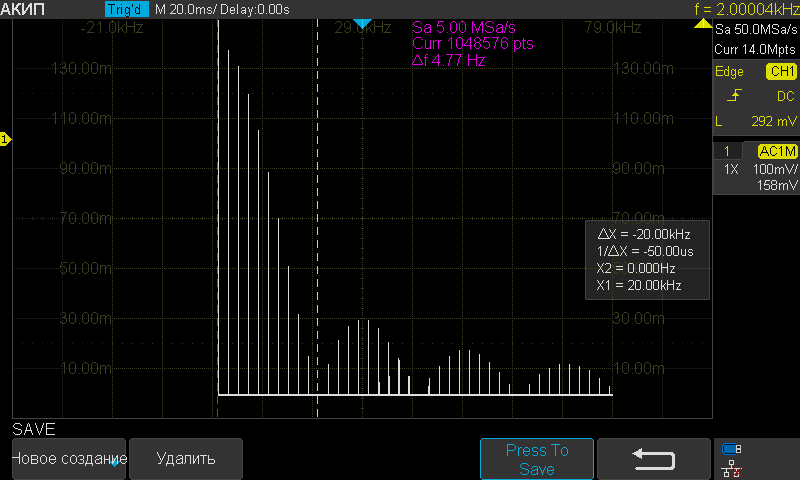
\includegraphics[width=0.9\linewidth]{"../photos/impulse2.png"}
		\vspace*{-5pt}
		\caption*{$\nu_T= 2$ кГц}
		\vspace*{-10pt}
	\end{minipage}
\end{figure}
\begin{figure}[H]
	\centering
	\begin{minipage}[b]{.5\textwidth}
		\vspace*{-15pt}
		\centering
		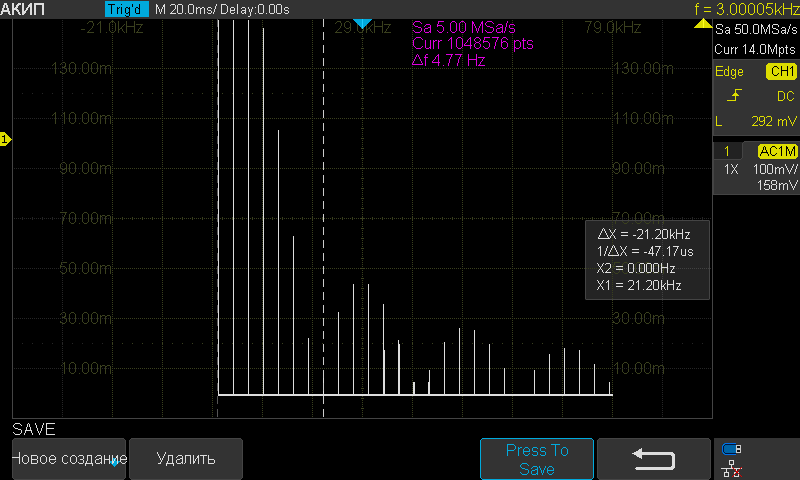
\includegraphics[width=0.9\linewidth]{"../photos/impulse3.png"}
		\vspace*{-5pt}
		\caption*{$\nu_T= 3$ кГц}
		\vspace*{-10pt}
	\end{minipage}%
	\begin{minipage}[b]{.5\textwidth}
		\vspace*{-15pt}
		\centering
		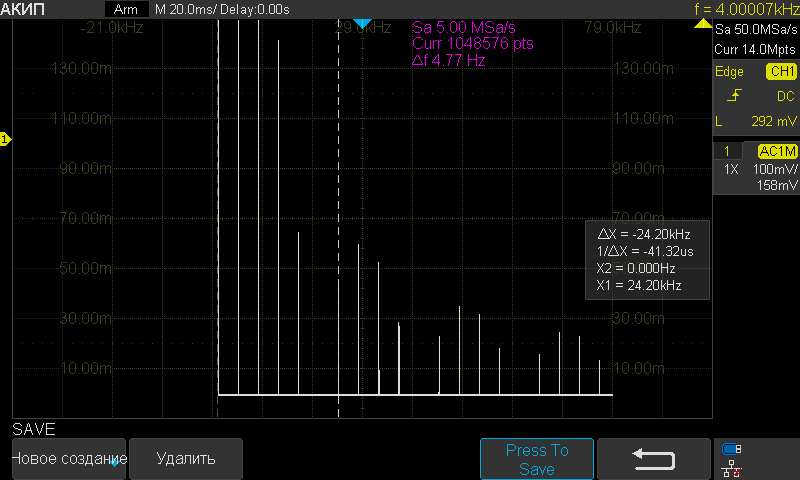
\includegraphics[width=0.9\linewidth]{"../photos/impulse4.png"}
		\vspace*{-5pt}
		\caption*{$\nu_T= 4$ кГц}
		\vspace*{-10pt}
	\end{minipage}
	\caption{Изменения спектра при увеличении $\nu$}
	\label{photo:impulse_nu}
\end{figure}

На снимках \ref{photo:impulse_tau} спектры при различных $\tau$. Изменение $\tau$ влияет только на ширину спектра.

\begin{figure}[H]
	\centering
	\begin{minipage}[b]{.5\textwidth}
		\vspace*{-10pt}
		\centering
		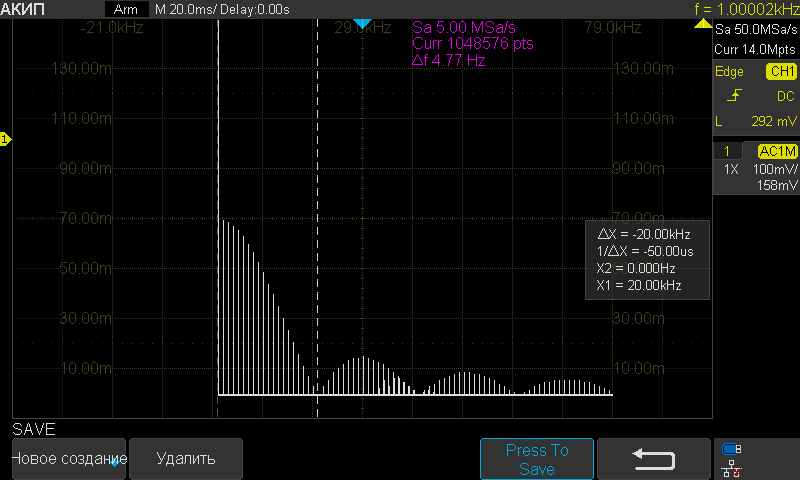
\includegraphics[width=0.9\linewidth]{"../photos/impulse1.png"}
		\caption*{$\tau = 50$ мкс}
		\vspace*{-20pt}
	\end{minipage}%
	\begin{minipage}[b]{.5\textwidth}
		\vspace*{-10pt}
		\centering
		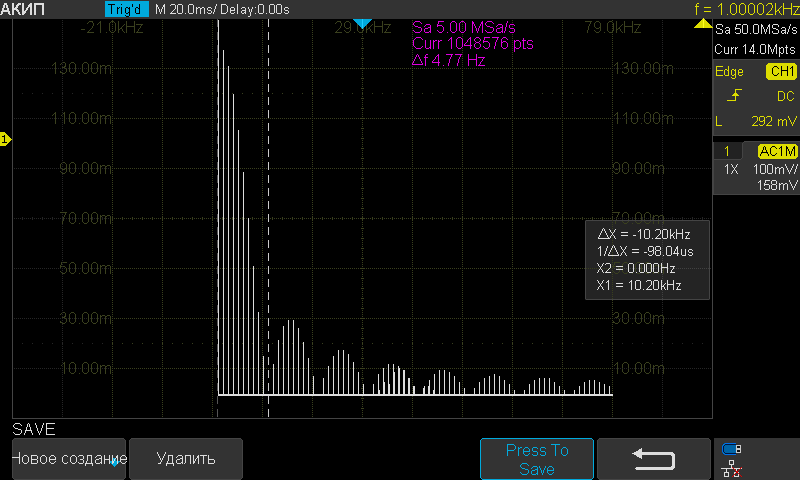
\includegraphics[width=0.9\linewidth]{"../photos/impulse5.png"}
		\caption*{$\tau = 100$ мкс}
		\vspace*{-20pt}
	\end{minipage}
\end{figure}

\begin{figure}[H]
	\centering
	\begin{minipage}[b]{.5\textwidth}
		\centering
		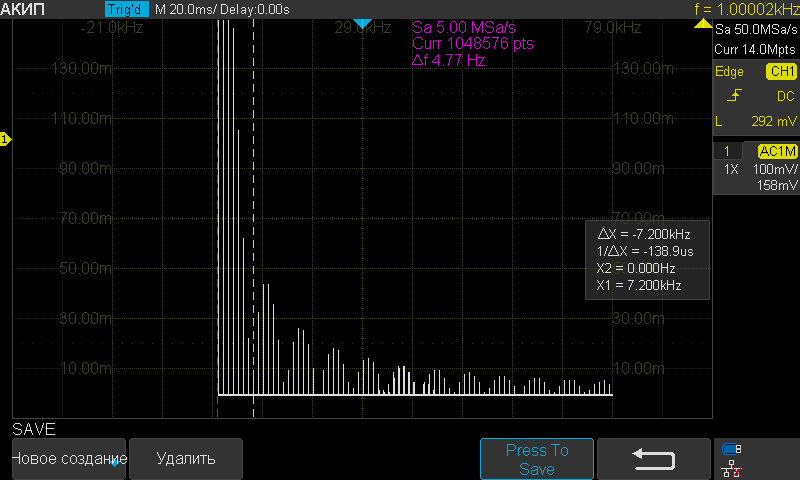
\includegraphics[width=0.9\linewidth]{"../photos/impulse6.png"}
		\caption*{$\tau = 150$ мкс}
	\end{minipage}%
	\begin{minipage}[b]{.5\textwidth}
		\centering
		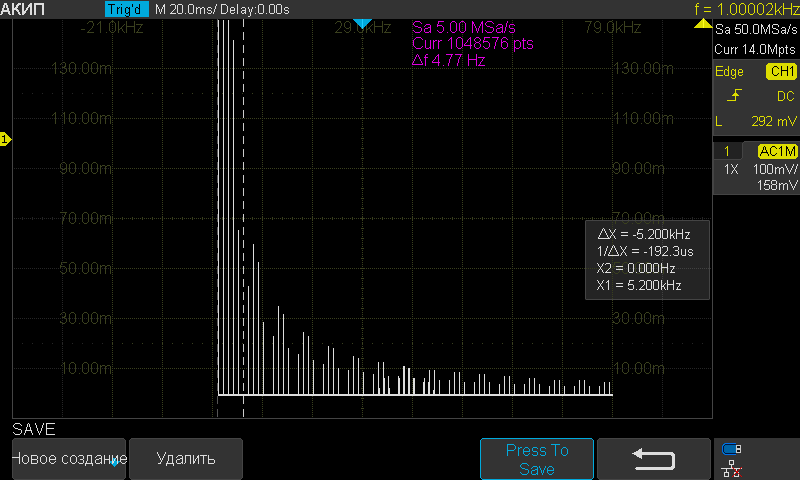
\includegraphics[width=0.9\linewidth]{"../photos/impulse7.png"}
		\caption*{$\tau = 200$ мкс}
	\end{minipage}
	\caption{Изменения спектра при увеличении $\tau$}
	\label{photo:impulse_tau}
\end{figure}

Измерим высоты гармоник спектра при $\nu_T = 1 \; \text{кГц}$, $\tau = 100 \; \text{мкс}$. Снимок спектра приведен на рисунке \ref{photo:harmonics}, график измеренных значений и огибающая приведены на рисунке \ref{fig:harmonics}. Теоретическая огибающая рассчитана по формуле:
$$ a_n = \frac{\sin{\pi n \tau / T}}{\pi n}. $$
 Нормировка $a_n$ проведена по высоте пика спектра.

\begin{figure}[H]
\begin{minipage}[H]{.5\textwidth}
		\vspace*{-15pt}
		\centering
		\includegraphics[width=1.0\linewidth]{"../gen/fig-a9.pdf"}
		\caption{Спектр и огибающая}
		\label{fig:harmonics}
\end{minipage}%
\begin{minipage}[H]{.5\textwidth}
		\centering
		\includegraphics[width=1.0\linewidth]{"../photos/impulse5"}
		\caption{Снимок экспериментального спектра}
		\label{photo:harmonics}
\end{minipage}
\end{figure}

Проверим выполнимость соотношения неопределенностей $\Delta \nu \cdot \tau = 1$. Для этого измерим зависимость ширины спектра $\Delta \nu(\tau)$ при постоянной $\nu_T = 1$ кГц.

\begin{figure}
\begin{minipage}[H]{.5\textwidth}
	\begin{figure}[H]
		\centering
		\includegraphics[width=1.2\linewidth]{"../gen/fig-a11.pdf"}
		\label{fig:a11}
	\end{figure}
\end{minipage}%
\begin{minipage}[H]{.5\textwidth}
	\begin{table}[H]
		\centering
		\input{../gen/tab-a11.tex}
	\end{table}
\end{minipage}
\vspace*{-20pt}
\caption{График зависимости $\Delta\nu(\frac{1}{\tau})$ }
\label{tab:a11}
\end{figure}

\begin{table}[H]
	\centering
	\input{../gen/tab-a11-mnk.tex}
	\caption{Обработка МНК}
	\label{tab:a11-mnk}
\end{table}


Погрешность эксперимента коррелирует с погрешностью коэффициента наклона. Следовательно, рассчитаем количественный критерий точности:

$$\mathcal{C} \approx \frac{\Delta a}{a} \approx 0.5 \% $$

\subsection*{Cпектр периодической последовательности синусоидальных цугов}

Теоретическое описание спектра периодической последовательности цугов приведено на рисунке \ref{res:zug}.

\begin{figure}[H]
	\centering
	\begin{minipage}[b]{.49\textwidth}
		\centering
		\includegraphics[width=0.9\linewidth]{"../res/zug"}
	\end{minipage}%
	\begin{minipage}[b]{.49\textwidth}
		\centering
		\includegraphics[width=0.9\linewidth]{"../res/zug_spectrum"}
	\end{minipage}
	\caption{Периодическая последовательность импульсов и её спектр.}
	\label{res:zug}
\end{figure}

На вход осциллографа подаем последовательность цугов. Период повторения $T = 1 \; \text{мс}$ ($\nu_T = 1 \; \text{кГц}$), число периодов в одном импульсе $N = 5$ (длительность импульса $\tau = N/\nu_{0} = 100$ мкс). Несущие частоты возьмем $\nu_0 = \{50, 70, 90\} \; \text{кГц}$. Снимки приведены на рисунке \ref{photo:zug}.

\begin{figure}[H]
	\centering
	\begin{minipage}[b]{.33\textwidth}
		\centering
		\includegraphics[width=0.9\linewidth]{"../photos/zug1"}
	\end{minipage}%
	\begin{minipage}[b]{.33\textwidth}
		\centering
		\includegraphics[width=0.9\linewidth]{"../photos/zug2"}
	\end{minipage}%
	\begin{minipage}[b]{.33\textwidth}
		\centering
		\includegraphics[width=0.9\linewidth]{"../photos/zug3"}
	\end{minipage}
\caption{Изменение спектра при увеличении несущей частоты}
\label{photo:zug}
\end{figure}

На снимках видно, что при увеличении несущей частоты спектр сдвигается, при этом центр спектра находится в $\nu_0$, это характерное отличие последовательности синусоидальных цугов от прямоугольных импульсов. На изменения $T$, $\tau$ спектр реагирует аналогично \ref{photo:impulse_nu}, \ref{photo:impulse_tau}.

Проверим выполнимость соотношения неопределенностей для $T$: $\delta \nu \cdot T = 1$. Для этого измерим зависимость $\delta \nu(T)$.

\begin{figure}[H]
	\begin{minipage}[H]{.5\textwidth}
		\begin{figure}[H]
			\centering
			\includegraphics[width=1.2\linewidth]{"../gen/fig-b16.pdf"}
			\label{fig:b16}
		\end{figure}
	\end{minipage}%
	\begin{minipage}[H]{.5\textwidth}
		\begin{table}[H]
			\centering
			\input{../gen/tab-b16.tex}
		\end{table}
	\end{minipage}
	\vspace*{-20pt}
	\caption{График зависимости $\Delta\nu(\frac{1}{\tau})$ }
	\label{tab:b16}
\end{figure}

\begin{table}[H]
	\centering
	\input{../gen/tab-b16-mnk.tex}
	\caption{Обработка МНК}
	\label{tab:b16-mnk}
\end{table}

Оценим погрешность как
$$\mathcal{C} \approx \frac{\Delta a}{a} \approx 1.0 \%.$$

\subsection*{Спектр гармонических сигналов, модулированных по амплитуде}

Теоретическое описание гармонического сигнала, модулированного по амплитуде приведено на рисунке \ref{res:am}.

\begin{figure}[H]
	\centering
	\begin{minipage}[b]{.49\textwidth}
		\centering
		\includegraphics[width=0.9\linewidth]{"../res/am"}
	\end{minipage}%
	\begin{minipage}[b]{.49\textwidth}
		\centering
		\includegraphics[width=1.0\linewidth]{"../res/am_spectrum"}
	\end{minipage}
	\caption{Амплитудная модуляция и её спектр.}
	\label{res:am}
\end{figure}

Настраиваем генератор на частоту несущей $\nu_{0} = 50 \; \text{кГц}$, частоту модуляции
$\nu_{\text{мод}} = 4 \; \text{кГц}$ и глубину модуляции $m = 0.5$. Частоты модуляции возьмем $\nu_{\text{мод}} = \{4, 8, 12\}$ кГц. Фотографии экрана электронного осциллографа приведены на рисунке \ref{photo:am}.	

\begin{figure}[H]
	\centering
	\begin{minipage}[b]{.33\textwidth}
		\centering
		\includegraphics[width=0.9\linewidth]{"../photos/am1"}
	\end{minipage}%
	\begin{minipage}[b]{.33\textwidth}
		\centering
		\includegraphics[width=0.9\linewidth]{"../photos/am2"}
	\end{minipage}%
	\begin{minipage}[b]{.33\textwidth}
		\centering
		\includegraphics[width=0.9\linewidth]{"../photos/am3"}
	\end{minipage}
	\caption{Изменения спектра при увеличении $\nu_{\text{мод}}$}
	\label{photo:am}
\end{figure}

Меняя на генераторе глубину модуляции $m$ в диапазоне от $10\%$ до
$100\%$, измерим отношение $\frac{a_{\text{бок}}}{a_{\text{осн}}}$ амплитуд боковой и основной спектральных линий. Строим график зависимости $\frac{a_{\text{бок}}}{a_{\text{осн}}}(m)$ (см. рис. \ref{fig:v21}).

\begin{figure}[H]
	\begin{minipage}[B]{.5\textwidth}
			\centering
			\includegraphics[width=1.1\linewidth]{"../gen/fig-v21.pdf"}
	\end{minipage}%
	\begin{minipage}[B]{.5\textwidth}
		\begin{table}[H]
			\centering
			\footnotesize
			\input{"../gen/tab-v21.tex"}
		\end{table}
	\end{minipage}
	\caption{График зависимости $\frac{a_{\text{бок}}}{a_{\text{осн}}}(m)$}
	\label{fig:v21}
\end{figure}


\begin{table}[H]
	\centering
	\footnotesize
	\input{"../gen/tab-v21-mnk.tex"}
	\caption{Обработка МНК}
	\label{tab:v21-mnk}
\end{table}

Погрешность эксперимента коррелирует с погрешностью коэффициента наклона. Следовательно, рассчитаем количественный критерий точности:

$$\mathcal{C} \approx \frac{\Delta a}{a} \approx 3 \% $$

